\documentclass[a4paper,12pt,oneside]{book}
\linespread{1.5}
\usepackage{geometry}
\geometry{top=3cm,bottom=3cm,left=3.5cm,right=3.5cm}
\usepackage[utf8]{inputenc}
\usepackage{tikz,pgf}
\usepackage{indentfirst}
\usepackage{amsfonts}
\usepackage[italian]{babel}

\usepackage{listings}
\usepackage{todonotes}
\usepackage{subfig}
\usepackage{fancyhdr}
\setlength{\parindent}{1cm}
\usepackage{graphicx}
\usepackage{float}
\usepackage{csquotes}
\usepackage{amsmath}
\usepackage{numprint}
\usepackage{pgfplots}
\usepackage{pgfplotstable}
\usepackage{tocbibind}
\usepackage{url}

\graphicspath{{images/}}

\setlength {\marginparwidth }{2cm} 
\pgfplotsset{compat=1.16}

\newenvironment{dedication}
  {\clearpage               % we want a new page
   \thispagestyle{empty}    % no header and footer
   \vspace*{\stretch{1}}    % some space at the top 
   \itshape                 % the text is in italics
   \raggedleft              % flush to the right margin
  }
   {\par % end the paragraph
   \vspace{\stretch{3}} % space at bottom is three times that at the top
   \clearpage           % finish off the page
  }
  
\begin{document}
%% Frontespizio %%
\begin{titlepage}
    \begin{center}
        \LARGE{\uppercase{\textbf{Università della Calabria}}}\\
        \vspace{5mm}
%% Dipartimento %%
    	\uppercase{\normalsize Dipartimento di Matematica e Informatica}\\
    \end{center}
    \begin{figure}[H]
        \centering
        
\includegraphics[width=0.7\textwidth]{images/logo.png}
    \end{figure}
    
    \begin{center}
%% Corso di Laurea %%
    	\large{ Corso di Laurea in Informatica}\\
    	\vspace{7mm}
%% Titolo della Tesi %%
        {\LARGE{\bf ERI Computer Assistant}}\\
    	\vspace{3mm}
    \end{center}
     
    \vspace{15mm}
    \noindent
    \begin{minipage}[t]{0.50\textwidth}
%% Relatore %%
    	{\large{ Relatore:\\\bf Prof. Mario Alviano\\}}
    	\vspace{12mm}

    \end{minipage}
    \hfill
    \begin{minipage}[t]{0.4\textwidth}\raggedleft
%% Candidato %%
    	{\large{Candidato: \\ \bf Alessandro Fazio\\ Mat. 200771}}
    \end{minipage}
    
    \vspace{20mm}
    
%% Anno Accademico %%
    \centering{\large \uppercase{ Anno Accademico 2020/2021}}

\end{titlepage}

% \begin{dedication}
%     "Because of the uproar over 2B’s butt,

%     there are loads of rude drawings and whatnot being uploaded [online]. 
    
%     And since going around and collecting them is a pain, 
    
%     I’d like it if I could get them sent in a zip file every week."

%     (Yoko Taro)
    
    
%     "Ulle Tulle"

%     (Antonio Norman Russo)
% \end{dedication}

%% Corpo della tesi %%

\chapter*{Sommario} %% In questa zona inseriamo l'abstract del nostro documento. %%
In questo lavoro di tesi è stato progettato e implementato un software che permette all'utente di interagire con il proprio sistema operativo Windows impartendo comandi vocali o testuali remotamente attraverso dispositivi compatibili con Google Assistant. 
Tale software si pone l'obiettivo di permette all'utente di controllare l'avvio e la chiusura di alcuni programmi di uso comune e di gestire il volume e la riproduzione di file multimediali. 
È stata inoltre resa possibile l'estensione delle funzionalità dell'assistente virtuale attraverso l'esecuzione di script python personali, incrementando così i potenziali utilizzi creando una esperienza personalizzabile e specifica. 

%\tableofcontents
%\listoffigures
\chapter{Introduzione}
\section{Contesto e Motivazione}
I primi personal computer necessitavano di una conoscenza specifica del modo di interagire con il sistema operativo. 
Erano molto specifici nei loro utilizzi e offrivano una interfaccia a linea di comando non neccessariamente user-friendly. 
Fortunatamente lo sviluppo di nuove tecnologie e la popolarità dei computer hanno spinto l'industria ad abbassare il livello di expertise necessario.
I sistemi operativi moderni consentono all'utente di interagire attraverso diverse modalità permettendo a diversi tipi di utente di approcciarsi come meglio credono.
Nonostante Windows sia il sistema operativo più diffuso in ambiente desktop, il suo assistente vocale, Cortana, offre un insieme ridotto di funzionalità, soprattutto se confrontanto con prodotti simili disponibili in altri sistemi operativi.
Assistenti vocali come Google Assistant per Android, e Siri per iOS permettono di controllare impostazioni del dispositivo su cui si trovano, rispondono alle domande dell'utente, e permettono di avviare attività. Tali funzionalità non sono presenti in Cortana.

\section{Obiettivi}
L'obiettivo di questo lavoro di tesi è appunto l'implementazione alcune di queste funzionalità mancanti. In particolare, attraverso l'assistente, l'utente potrà eseguire i seguenti comandi:

\begin{itemize}
    \item Avvio di programmi installati
    \item Chiusura di programmi in esecuzione
    \item Controllo del volume del dispositivo
    \item Controllo della riproduzione di file multimediali
    \item Esecuzione di routine create dall'utente tramite python
\end{itemize}

\section{Contributo principale}
Più precisamente, il client permette di eseguire azioni automaticamente impartendo remotamente comandi attraverso un altro dispositivo.
Questo è possibile grazie all'implementazione di una "Azione per Google Assistant" in grado di convertire voce o testo in un comando comprensibile dal client in esecuzione sul dispositivo che si vuole controllare.
È stato scelto questo approccio remoto per permettere all'utente di controllare il dispositivo anche senza avere accesso fisico al dispositivo.
\subsubsection{Struttura del lavoro di tesi}
La presentazione di questo lavoro di tesi è strutturata nel seguente modo:

Il Capitolo 2 mostra le principali tecnologie utilizzate con un esempio generico di utilizzo, introducendo i principali concetti di programmazione legati ad essi.

Il Capitolo 3 contiene una panoramica generale dell'assistente comprensivo di struttura del progetto, principali implementazioni, ed eventuali problemi riscontrati durante lo sviluppo.

Il Capitolo 4 espone alcune possibili soluzioni a dei problemi esposti nel capitolo precedente.

Il Capitolo 5 conclude l'esposizione introducendo alcuni suggerimenti e possibili miglioramenti.

\section{Problemi tecnici riscontrati}
\label{sec:problematecnico}
Il progetto utilizza Google Assistant, attualmente disponibile solo su dispositivi Android, questo significa che non è stato possibile implementare una soluzione nativa a Windows. 
A causa di questa limitazione è stato necessario implementare un client nativo che si collega ad un back-end esterno, in questo caso, Firebase. 
Grazie Firebase però, è stato possibile semplificare l'architettura del sistema visto che è una piattaforma di Backend-As-a-Service molto in voga. 
Grazie a Firebase è stato possibile utilizzare un sistema di autenticazione e un database già implementati e testati da esperti del settore, il che allegerisce il carico di molto. 
Inoltre, per alcune funzionalità implementate è stato necessario utilizzare alcune API Windows tramite python poichè non esistono in Javascript, il che porta dunque ad una ulteriore dipendenza per il corretto funzionamento del software.  % rivedere
\chapter{Tecnologie Utilizzate}
\label{cap:tecnologie}

In questo capitolo verranno descritte le tecnologie utilizzate nella realizzazione del progetto.

\section{HTML e CSS}
\subsection{HTML}
HTML, o HyperText Markup Language, è un liguaggio che permette di creare pagine web definendone la struttura, la quale verrà successivamente interpretata dal browser, principale strumento per la fruizione di pagine web.
Una pagina HTML è composta da elementi creati attraverso i cosiddetti tag html.
La struttura base di una pagina HTML è formata da 1 tag principale chiamato $<html>$  che conterrà altri 2 tag fondamentali, $<head>$  e $<body>$.
Nel tag $<head>$  si inseriranno informazioni non visibili nella pagina mostrata dal browser (fatta eccezione per il titolo della pagina), mentre nel $<body>$  andremo ad inserire tutto quello che l'utente andrà a vedere e con il quale potrà interagire.
Vediamo un esempio:
\begin{figure}[H]
    \centering
    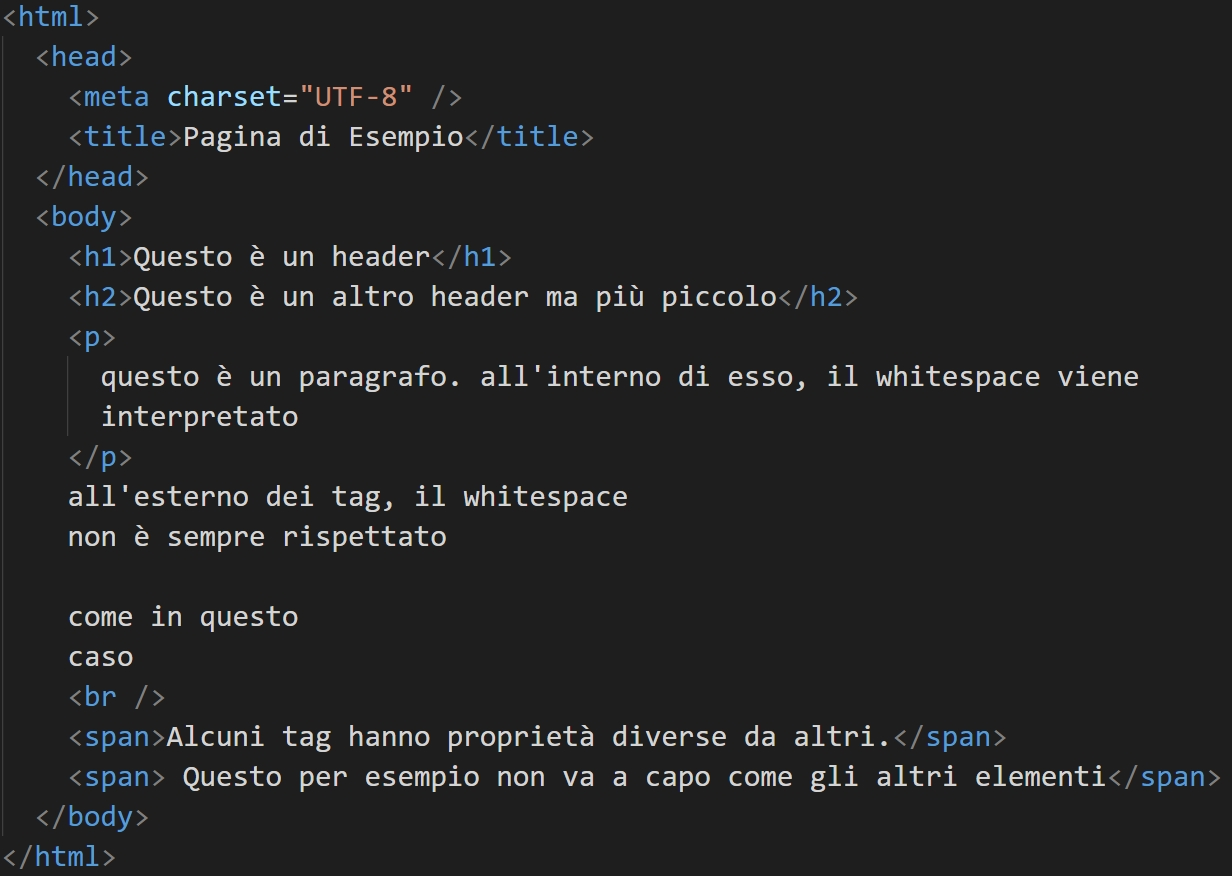
\includegraphics[scale=0.45]{images/html_code_example.jpg}
    \caption{Codice sorgente HTML}
    \label{fig:codice_html}
\end{figure}
\begin{figure}[H]
    \centering
    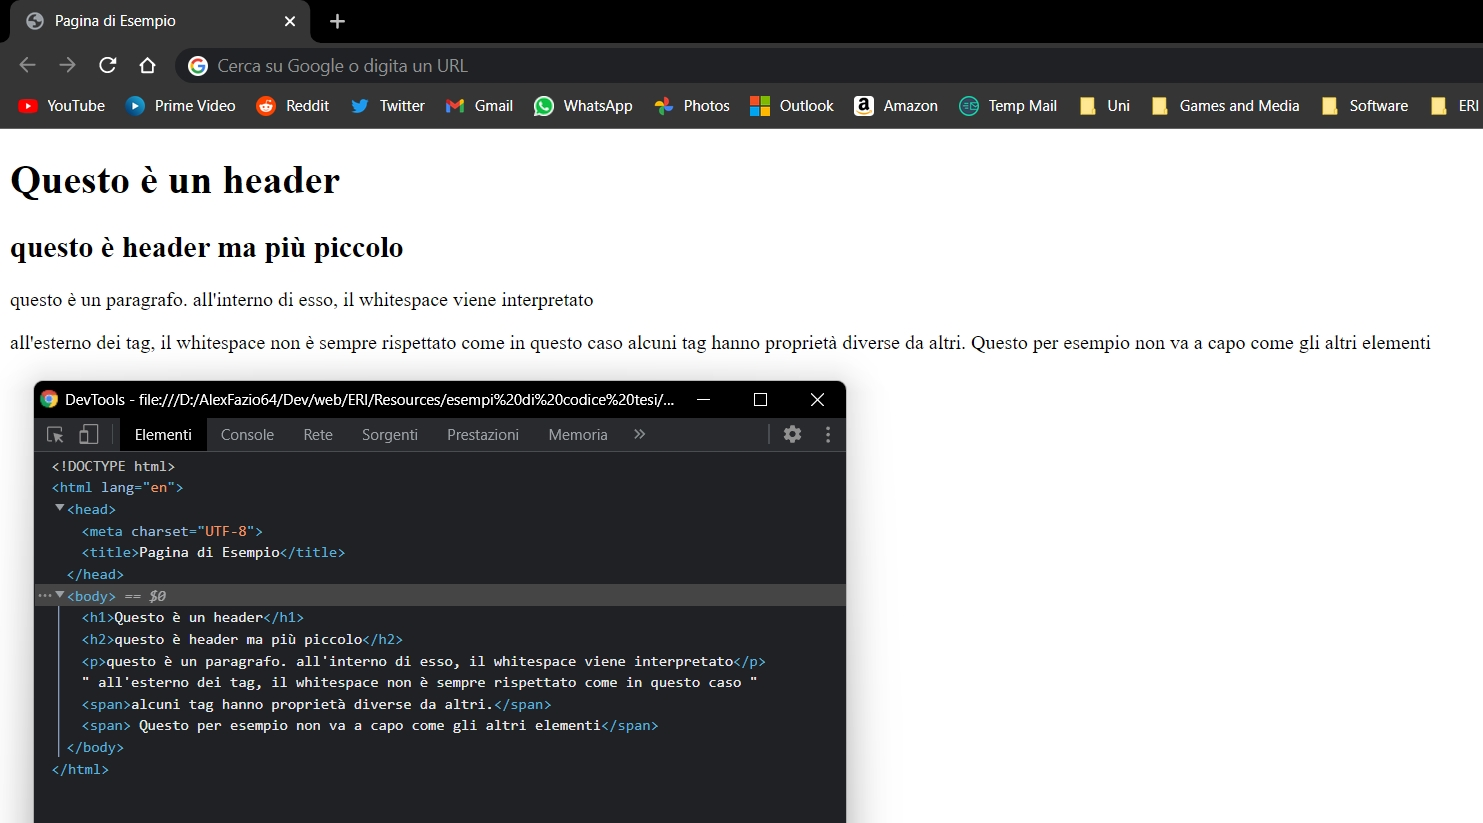
\includegraphics[scale=0.4]{images/browser_interpretation.jpg}
    \caption{Pagina web interpretata dal browser}
    \label{fig:pagina_nel_browser}
\end{figure}
HTML rende possibile la creazione di una pagina interattiva basilare, ma grazie a linguaggi di supporto quali CSS e Javascript è possibile stilizzare il contenuto ed eventualmente cambiare il comportamento standard degli elementi.
\subsection{CSS}
CSS, acronimo di Cascading StyleSheets permette di personalizzare il modo in cui il browser mostra il contenuto della pagina HTML al quale viene applicato.
Vengono introdotti nuovi concetti in modo da applicare lo stile selettivamente.
Concetti come regole, proprietà e selettori rendono possibile specificare uno stile diverso da quello di default del browser. Vediamo un esempio:
\begin{verbatim}
    p {
        color: red;
        font-size: 24pt;
        color: green;
    }
\end{verbatim}
In questo spezzone di codice è rappresentata una regola.
\begin{itemize}
    \item p è un selettore che identifica ogni tag $<p>$  indistintamente
    \item color e font-size delle proprietà
    \item red, 24pt e green sono valori
\end{itemize}
Questa regola renderà ogni paragrafo di colore verde e con font impostato a 24pt, questo poichè le regole e le proprietà vengono applicate a cascata (Cascading appunto).
Dato che color viene ridefinita più volte, l'ultima definizione avrà la priorità.

\section{Javascript e Typescript}
\subsection{Javascript}
Javascript è un linguaggio di scripting utilizzato principalmente per lo sviluppo di applicazioni web.
Grazie ad esso è possibile rendere dinamiche le pagine web reagendo alle azioni dell'utente.
Rende possibile modificare il comportamento standard degli elementi interattivi nelle pagine.
E' un linguaggio basato su multipli paradigmi, interpretato, debolmente tipizzato.
Tutti i browser moderni permettono alle pagine web di eseguire codice Javascript in un ambiente isolato, ovvero, ogni pagina può eseguire il proprio codice ma senza accedere al codice di altre pagine.
Esistono vari modi di includere codice Javascript all'interno di pagine html, ma il più comune è quello di importare il file .js all'interno di un tag $<script>$.
\subsection{Typescript}
Typescript è una versione tipizzata di Javascript, come suggerisce il nome.
Segue tutte le regole dello standard Javascript, ma rende più semplice l'implementazione e il debugging del codice da parte dello sviluppatore grazie a strumenti integrati negli ambienti di sviluppo.
I browser però non riescono ad interpretare codice scritto in Typescript dato che ha una notazione diversa, c'è quindi bisogno di tradurre tale prodotto in codice Javascript valido, e questo passo è fortunatamente automatizzato grazie a software appositi.

\section{Python}
Python è un liguaggio ad alto livello, interpretato e multiparadigma.
E' un linguaggio multiuso con il quale si possono implementare applicazioni di ogni tipo.
E' caratterizzato dalla somiglianza al linguaggio naturale e dalla sua notazione minimale che enfatizza la semplicità di implementazione.
E' stato scelto il suo utilizzo nel progetto proprio per la sua immediatezza e semplicità.

\section{Firebase}
Firebase è un servizio di Backend-as-a-Service (BaaS) offerto da Google.
Fornisce librerie in diversi linguaggi per intergrare tale servizio nelle applicazioni.
Tra i principali servizi offerti e utilizzati nel progetto abbiamo un Database Realtime e il servizio di Autenticazione.
Tali servizi sono già implementati e testati da esperti del settore in modo tale da semplificare il lavoro agli sviluppatori, i quali potranno usufruirne gratuitamente o a pagamento, ovviamente con ulteriori benefici e servizi avanzati.
Questo lavoro di tesi utilizza il piano gratuito offerto da Firebase poichè non si è necessitato di ulteriori funzionalità e dove necessario si è utilizzata una alternativa gratuita sfruttando un altri servizi.

\subsection{Realtime Database}
Il Realtime Database offerto da Firebase è un database JSON (JavaScript Object Notation) ottimizzato in modo tale da avere un bassissima latenza.
E' stato scelto tale database poichè i dati necessari al funzionamento della applicazione sono rappresentabili facilmente come JSON, e la bassa latenza aiuta con la reattività dell'assistente virtuale data la sua natura conversazionale.

\section{Svelte}
Svelte è un compilatore in grado di generare applicazioni web collegando la logica alla grafica attraverso una sintassi simile ad HTML e Javascript.
Permette allo sviluppatore di scrivere meno codice rispetto all'approccio tradizionale, e lo fa estendendo la sintassi standard in modo da rimanere familiare, ma introducendo concetti che facilitano lo sviluppo.
Svelte è basato su un approccio a componenti riutilizzabili. La struttura tipica di un componente è la seguente:

\begin{itemize}
    \item un tag $<script>$ locale al componente, all'interno del quale possiamo specificare la logica
    \item un tag $<style>$ dove possiamo personalizzare il modo in cui esso viene renderizzato dal browser
    \item una sezione in cui possiamo includere i tag standard di HTML
\end{itemize}

Il principale vantaggio di utilizzare Svelte è, come già accennato, il binding tra logica e grafica, e la semplicità con il quale viene realizzato.
\subsection{Frameworks}
Tradizionalmente per cambiare il comportamento di un bottone sono necessari 3 file diversi, un file .html dove definiamo la struttura della pagina, un file .js nel quale andiamo a selezionare il bottone in maniera molto verbosa, e un file .css dove personalizziamo lo stile di tale bottone.
Con Svelte basta un solo file .svelte che verrà successivamente compilato in diversi file a seconda delle funzionalità implementate.
Esistono altri strumenti, anche chiamati framework, simili a Svelte che permettono di sviluppare webapp facilitando il lavoro dello sviluppatore, per esempio:

\begin{itemize}
    \item React
    \item Vue
    \item Angular
    \item molti, molti altri\dots
\end{itemize}

Si è scelto di utilizzare Svelte per la realizzazione dell'interfaccia, per la quantità minimale di codice boilerplate necessaria rispetto ad altri framework, la leggibilità, le alte prestazioni e il supporto nativo a Typescript.

\begin{figure}[H]
    \centering
    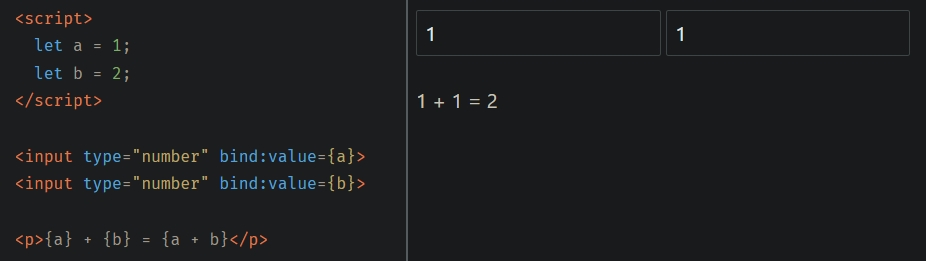
\includegraphics[scale=0.7]{images/svelte_example.jpg}
    \caption{Esempio di applicazione Svelte che sincronizza i valori di 2 $<input>$ sommandoli e stampandoli in un paragrafo }
    \label{fig:svelte_example}
\end{figure}
\begin{figure}[H]
    \centering
    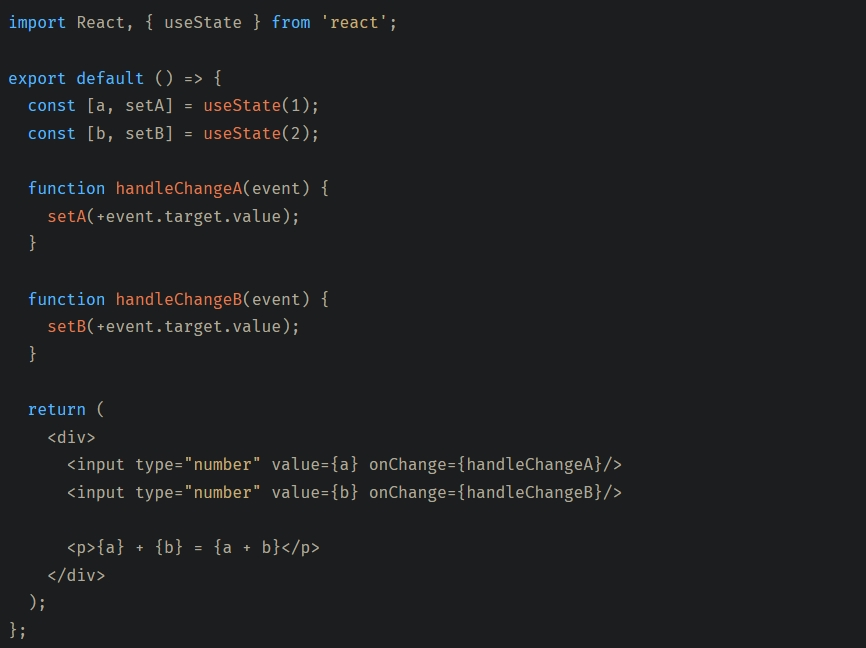
\includegraphics[scale=0.7]{images/react_example.jpg}
    \caption{La stessa applicazione ma scritta in React}
    \label{fig:react_example}
\end{figure}
\begin{figure}[H]
    \centering
    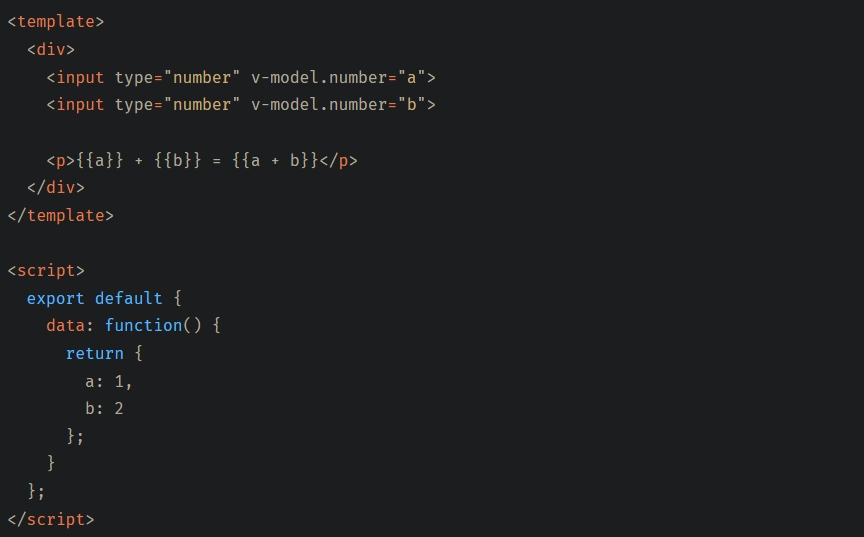
\includegraphics[scale=0.7]{images/vue_example.jpg}
    \caption{La stessa applicazione ma scritta in Vue}
    \label{fig:vue_example}
\end{figure}
\textbf{N.B:} esempi di codice presi da svelte.dev

\section{Sveltekit}
Sveltekit è un framework che include Svelte ed aggiunge ulteriori funzionalità com.



Sveltekit è un framework basato su Svelte che permette di creare applicazioni web fornendo un’esperienza di sviluppo più comoda e rapida. Diversamente dalle altre applicazioni basate su server side rendering, SvelteKit rende l’esperienza più rapida e fluida. \'E basato su Snowpack, un tool che velocizza il processo di sviluppo, compilando i file una singola volta e, successivamente, ricompilandoli solamente in caso di cambiamenti all'interno del codice. Il punto di forza di Sveltekit è la possibilità di avere un routing delle pagine basato sul file-system; ciò significa che la struttura dell’applicazione è basata sulla struttura del codice. Quindi, come per React, non c’è bisogno di utilizzare un router esterno per la propria applicazione web, come ad esempio Redux. Le funzionalità di Sveltekit sono numerose e la principali utilizzate in questo progetto sono state il \textit{server-side rendering} e il \textit{routing dinamico}.

\section{NodeJS e NPM}
\subsection{NodeJS}
NodeJS (o più semplicemente, Node) è una implementazione di ambiente runtime per Javascript basato su V8, l'ambiente runtime presente sul browser Chrome.
Permette di eseguire codice Javascript senza necessità di un browser.
Questo permette a Javascript di diventare un linguaggio multifunzione con la possibilità di realizzare applicazioni non per forza legate all'ambiente web.
Node aggiunge fornisce altre funzionalità, come l'interazione con il sistema operativo sul quale viene eseguito, il che lo rende il candidato perfetto per questo tipo di progetto.

\subsection{Node Package Manager}
NPM è un gestore di pacchetti per Javascript ed è il gestore di pacchetti predefinito su Node.
Un pacchetto software, in generale, è un insieme di programmi distribuiti congiuntamente che risolvono un problema specifico, in questo caso, un insieme di file Javascript correlati tra loro.
Con NPM è possibile integrare pacchetti realizzati da altri utenti nel proprio progetto, semplificando l'implementazione di funzionalità necessarie.
Un esempio di pacchetto utilizzato all'interno di questo progetto è appunto Firebase.

\section{Express}
Express JS

\section{Heroku}
Heroku

\section{Actions on Google}
Actions on Google
\subsection{Google Assistant}
Google Assistant
\subsection{Actions Console}
Actions Console
%\chapter{Contributo principale}

Obiettivo principale di questo progetto è, come detto in precedenza, permettere il controllo remoto di un dispositivo Windows attraverso l'interazione con Google Assistant.
L'utente avrà inoltre la possibilità di specificare quali programmi sarà possibile invocare ed eventualmente di specificare delle routine personalizzate attraverso la scrittura di script python.

In questa sezione verranno descritte le funzioni principali e le loro implementazioni tramite frammenti di codice e grafici.

\section{Panoramica e struttura dell'applicazione}
L'applicazione è divisa in tre sezioni principali le quali verranno trattate separatamente.

Le sezioni sono:
\begin{itemize}
    \item Front-end
    \item Assistente
    \item Back-end
\end{itemize}

\section{Front-end}
La parte front-end include l'interfaccia grafica realizzata in SvelteKit e l'applicativo Electron che la incapsula.
Gran parte del lavoro è stato quello di creare un sito web funzionante che permetta all'utente di effettuare il login con Google, e successivamente di collegare il tutto con Firebase e il realtime database.

SCREENSHOT ERI CLIENT

\subsection{Schermata di accesso}
\label{subs:profilo}
Il login è una parte principale della applicazione poichè è necessario che l'utente possa controllare solamente i propri dispositivi. Per fare ciò si è scelto di utilizzare firebase e il suo servizio di autenticazione. Dato che la registrazione a dall'utente può essere effettuata completamente a voce, si è scelto di utilizzare il tipo di accesso tramite OAuth.
OAuth è un tipo di flusso di autenticazione diverso da quello standard che richiede username e password. OAuth introduce dei concetti diversi per garantire la sicurezza. In primo luogo abbiamo i provider di sicurezza che immagazzinano tutte le informazioni confidenziali dell'utente, abbiamo poi le applicazioni di terze parti che richiedono l'accesso ad un profilo, e infine abbiamo i token di sicurezza, garantiti solo in caso di accesso corretto.
Quando un utente vuole effettuare l'accesso tramite una applicazione, esso viene reindirizzato ad una pagina di login sul server del provider di sicurezza. Questa pagina verrà generata on-demand e ad accesso effettuato, verrà reindirizzato sulla pagina al quale voleva accedere, con tutte le informazioni necessarie fornite dal provider. Tutto questo processo avviene secondo protocolli di comunicazione protetti minimizzando così il rischio di attacco.

GRAFICO OAUTH2 FLOW

SCREEN POPUP GOOGLE ERI

\subsection{Dashboard utente}
La pagina dell'utente permette di gestire la lista di programmi avviabili e di collegare il dispositivo a firebase in modo che possa ricevere comandi dall'assistente.
Nella parte superiore abbiamo l'identificativo dell'utente e del dispositivo. Nel caso in cui l'uuid non sia sincronizzato con il database, apparirà un tasto che permetterà di sincronizzarli.
L'applicazione rimane in ascolto dei cambiamenti del valore sul database e nel caso in cui non fossero uguali non eseguirà i comandi.

SCREEN sync button

Nella parte inferiore si trovano i componenti Svelte che permettono di specificare i programmmi da collegare all'applicazione.
Per fare ciò si è necessitato di una funzionalità fornita da Electron, ovvero un wrapper per la classe File di Javascript che permette di accedere al percorso completo del file.
Normalmente tale percorso è offuscato dai browser per motivi di sicurezza.
Per collegare un programma è necessario effettuare il trascinamento del programma sull'apposita icona.
L'icona ascolta l'evento \textit{drop} e tramite la funzione \textit{nome funzione} l'applicazione sarà in grado di estrarre il percorso dell'eseguibile indicato.

SCREEN ICONA + tooltip

Per rendere più affidabile tale funzione, è possibile trascinare anche i collegamenti all'eseguibile, questo poichè è più facile che l'eseguibile effettivo sia sempre in una posizione precisa, mentre è possibile che i collegamenti vengano spostati.
Nel caso in cui si trascinasse un collegamento, la funzione riesce ad estrarre il percorso del programma a cui punta il collegamento attraverso una serie di comandi disponibili nel cmd di Windows.
Oltre al percorso del programma, è necessario anche il nome effettivo del processo che viene avviato, solitamente uguale al nome dell'eseguibile, poichè la funzionalità di arresto dei programmi necessita del nome esatto del processo da stoppare.

SCREEN snippet codice

In fondo alla schermata si trova un bottone di salvataggio che permette di rendere persistente la mappa dei programmi cosicché l'utente non debba indicare ogni volta i percorsi dei programmi.
Quando il bottone viene cliccato, verrà scritto un file .json contenente tutti i percorsi indicati.
Ad ogni accesso dell'utente, tale file verrà letto, ripristinando tutti i percorsi precedentemente specificati.

SCREEN save button + screen file.json

\subsection{Funzioni di Firebase nel client}
\subsubsection{Struttura del rtdb}
\subsubsection{Lettura dei dati da Firebase}

\subsection{Funzionalità principali}
\subsubsection{Avvio di programmi}
\subsubsection{Chiusura di programmi}
\subsubsection{Controllo dei media}
\subsubsection{Routine personali}
\subsubsection{Problema tecnico}

\section{Assistente}
\subsection{Agenti}
\subsection{Struttura di una conversazione}
introduzione concetti necessari
\subsubsection{Autenticazione}
\subsubsection{Flusso standard}
collegamento al webhook da introdurre subito dopo

\section{Back-end}
\subsection{Webhook}
\subsection{Firebase}
\subsubsection{Firebase Auth}
\subsubsection{Realtime Database}

BIG GRAFICO ENORME OMMNICOMPRENSIVO DI TUTTO IN THE WORLD FOREVER
%\chapter{Discussione}

Questa sezione discute alcune funzionalità già descritte precedentemente, con l’obiettivo di illustrare i problemi che persistono nella loro attuale implementazione.
Verranno inoltre esposte alcune possibili soluzioni a questi problemi, unitamente a dei possibili miglioramenti apportabili in futuro.

\section{Problemi}
\subsection{Requisiti per l'utilizzo}
Il problema più evidente nel progetto è che non è una soluzione all-in-one poichè necessita che il sistema abbia Node e Python già installati e visibili nelle variabili di sistema.
Node è necessario a causa del fatto che SvelteKit non permette di compilare in una unica soluzione il sito sviluppato. Il sito sviluppato necessita di un cosiddetto adapter che fungerà da server. 
Python è invece necessario poichè le funzionalità che interagiscono con la libreria win32 utilizzata è implementata in python e tramite Electron viene invocato uno script python per interagire con tale API. 
Oltre a Python però, è necessaria l'installazione di tale api dato che non viene resa disponibile con la sola installazione dell'interprete python. 
Questo pone ovviamente un carico di lavoro eccessivo all'utente dato si necessita che il sistema sia ben configurato affinchè l'applicazione possa funzionare.

\subsection{User Experience}
Come già accennato, l'utente è il responsabile della configurazione corretta del software, processo che potrebbe essere automatizzato. 
Data la complessità nell'automatizzare il processo di mappatura dei programmi installati si è scelto l'approccio drag-and-drop per la categorizzazione dei programmi. 
Questo fornisce una maggiore flessibilità nella scelta, ma va in contrasto con la ragione per cui si è sviluppato tale applicativo, ovvero quella di offrire una interazione più semplice con il dispositivo. 

\subsection{Ambiguità nell'invocazione dei programmi}
A causa della grande mole di software diversi è stato necessario selezionare alcune delle categorie più comuni tra i programmi più popolari. 
Non è possibile chiedere all'assistente di avviare un programma specifico non presente nel dizionario configurato su Actions on Google. 
Un esempio di questo problema è una frase del genere:

\textit{Start IntelliJ IDEA}

L'assistente capisce che deve avviare un programma, ma dato che IntelliJ IDEA non presente nei \textit{types} dell'assistente nè come categoria, nè come alias, non è possibile estrapolare la categoria di software da avviare. 
\'E possibile però assegnare IntelliJ IDEA ad una categoria diversa nel client (ad esempio mappare IntelliJ alla categoria \textit{music}) oppure creare una routine personalizzata in python. 
Entrambe le soluzioni non sono molto intuitive in quanto la prima prevede di avviare un programma utilizzando un altro nome, e la seconda prevede di invocare un programma assegnando un numero al nome dello script che lo invoca.
\'E stato scelto di lasciare però tali possibilità agli utenti che ne potrebbero beneficiare.

\subsection{Deploy}
Il maggiore dei problemi è purtroppo l'effettiva pubblicazione dell'agente al pubblico. 
Attualmente l'agente è disponibile solamente attraverso l'account dello sviluppatore, quindi è possibile provare l'effettivo funzionamento dell'applicazione accedendo con quel profilo. 
Tutte le funzionalità sarebbero comunque disponibili a tutti gli utenti iscritti una volta pubblicato l'agente, ma al momento non è stato possibile rendere disponibile l'agente a tutti. 
Si è scelto di non pubblicare l'agente al momento poichè bisognerebbe stilare una privacy policy e dei termini di servizio compatibili con quelli richiesti da Google, ed al momento questo è fuori dallo scope del lavoro di tesi.

\section{Miglioramenti}
\subsection{Client nativo}
Date le elevate dimensioni dell'applicazione Electron, un miglioramento possibile è quello di reimplementare l'applicazione desktop utilizzando un linguaggio nativo per la costruzione di interfacce grafiche. 
C++ e la libreria wxWidgets sono degli ottimi candidati per il lavoro, e come ulteriore vantaggio avremmo la possibilità di interagire con le API windows per il controllo dei media senza l'utilizzo dell'interprete python eliminando 2 dipendenze.

\subsection{Integrazione di Google Assitant in Windows}
Esiste un progetto open source disponibile su Github che permette di interagire con Google Assistant direttamente da Windows attraverso una interfaccia grafica non ufficiale per Google Assistant.
Questo progetto permetterebbe di eliminare il requisito di utilizzo del dispositivo mobile per impartire comandi, rendendolo opzionale. 
Data la natura open source del progetto, sarebbe possibile integrare la logica di esecuzione dei comandi direttamente in un solo programma.
%\input{capitoli/capitolo5}

%\bibliographystyle{plain}
%\nocite{*}
%\bibliography{bibliografia.bib}

%Eliminare/Aggiungere/Personalizzare i capitolo nella cartella "capitoli"

%\chapter*{Conclusioni} In questo modo non comparirà dell'indice


\end{document}
